%!TEX program = pdflatex
\documentclass[10pt]{article}
\usepackage[pdftex]{graphicx, color}
\usepackage{listings}

\usepackage{tikz}
\usetikzlibrary{automata,positioning}

\headheight 8pt \headsep 20pt \footskip 30pt
\textheight 9in \textwidth 6.5in
\oddsidemargin 0in \evensidemargin 0in
\topmargin -.35in

\newcommand {\pts}[1]{({\bf #1 pts})}   
\lstset{basicstyle=\small\ttfamily,breaklines=true}

\begin{document}
\begin{center}
\Large CS131 Compilers: Writing Assignment 1\\Due Monday, September 30, 2019 at 22:00
\end{center}

\begin{center}
%% Change this:
\LARGE Name - ID
\end{center}


This assignment asks you to prepare written answers to questions on
regular languages, finite automata, and lexical analysis.  Each of the
questions has a short answer.  You may discuss this assignment with
other students and work on the problems together.  However, your
write-up should be your own individual work and you should indicate in your submission who you worked
with, if applicable.  Written assignments are turned in at the start of lecture.
You should use the Latex template provided at the course web site to write your solution and use the \emph{tikz} package to draw
automata.

\begin{center}
%% Change this:
I worked with: (zhanglw,2018533113)
\end{center}

\begin{enumerate}
  \item \pts{$2\times 3=6$} For each of the follow prompts, write any non-empty sentence:
  \begin{enumerate}

           \item Name one reason why you would like to learn in this class.
            \[
            For\,a \,wider \,knowledge\, in\, compiler\, and\, meeting\, great\, people\, in\, our\, school.  \]
           \item Write a question you would like the professor to answer on any topic, from personal opinions to the class material.
            \[
            Is\; that\; possible\; to\; invent\; EEG\; compiler?
            \]
           \item What do you expect from this class.
            \[
            A+
            \]

  \end{enumerate}
  %
  \item \pts{$2\times 4=8$} Write regular expressions for the following languages over the alphabet $\Sigma=\{0,1\}$:
 \begin{enumerate}
           \item $L_1$: The set of all finite strings containing at least three $1's$.
            \[
            %% Your answer here
				\Sigma^*1\Sigma^*1\Sigma^*1\Sigma^*
            \]
           \item $L_2$: The set of all finite strings containing at most two $0's$.
            \[
            %% Your answer here
				1^*\cup1^*01^*\cup1^*01^*01^*
            \]
           \item $L_3$: The set of all finite strings containing at most two $0's$ and at least three $1's$.
            \[
            %% Your answer here
				111^+\cup111^+0\cup11^+01^+\cup1^+011^+\cup0111^+\cup11^+001^+\cup1^+0011^+\cup00111^+\cup     \]
            \[
            \\ 01^+011^+\cup011^+01^+\cup0111^+0\cup1^+01^+01^+\cup1^+011^+0\cup11^+01^+0\cup111^+00
            \]
           \item $L_4$: The set of all finite strings containing at least three $1's$, but no two $1's$ appear consecutively.
            \[
            %% Your answer here
				0^*10^+1(0^+1)^+0^*
            \]
   \end{enumerate}
   This example illustrates that regular languages are closed under intersection. Note that
   $L_3=L_1\cap L_2$.

  \newpage
   \item \pts{$2\times 4=8$} Draw DFA's for each of the languages $L_1$, $L_2$, $L_3$ and $L_4$ from Question 2.
  \begin{enumerate}
    \item $L_1$.
    \\
    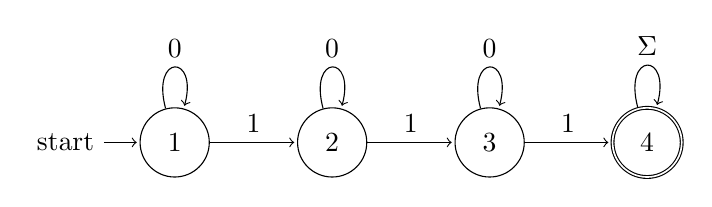
\begin{tikzpicture}[shorten >=1pt,node distance=2cm,on grid,auto]
        %% Your answer here
        \node[state,initial] (1)   {$1$};
        \node[state] (2) [right=of 1] {$2$};
        \node[state] (3) [right=of 2] {$3$};
        \node[state,accepting](4) [right=of 3] {$4$};
        \path[->]
        (1) edge [loop above] node {$0$} ()
            edge  node  {1} (2)
        (2) edge  node  {1} (3)
            edge [loop above] node {$0$} ()
        (3) edge  node  {1} (4)
            edge [loop above] node {$0$} ()
        (4) edge [loop above] node {$\Sigma$} ();

    \end{tikzpicture}
    \item $L_2$.
    \\
    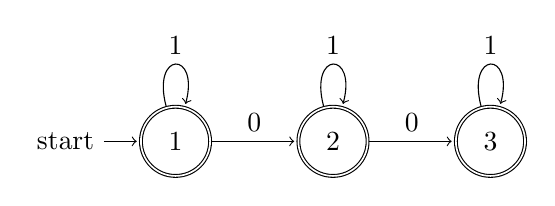
\begin{tikzpicture}[shorten >=1pt,node distance=2cm,on grid,auto]
        %% Your answer herez
        \node[state,initial,accepting] (1)   {$1$};
        \node[state,accepting] (2) [right=of 1] {$2$};
        \node[state,accepting] (3) [right=of 2] {$3$};
        \path[->]
        (1) edge [loop above] node {$1$} ()
            edge  node  {0} (2)
        (2) edge  node  {0} (3)
            edge [loop above] node {$1$} ()
        (3) edge [loop above] node {$1$} ();
    \end{tikzpicture}
    \item $L_3$.
    \\
    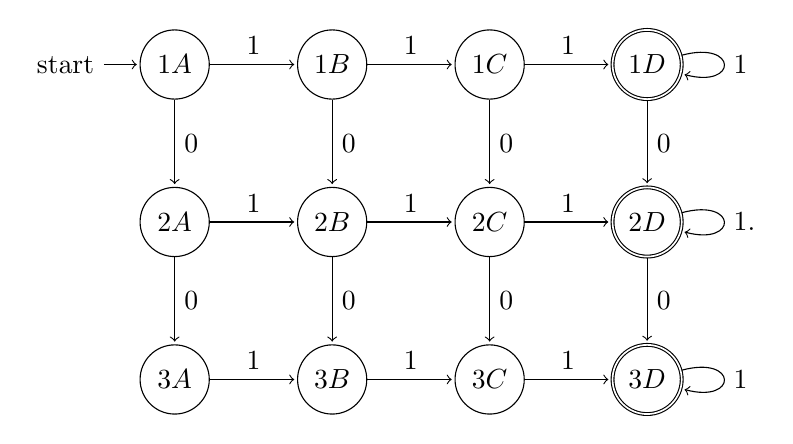
\begin{tikzpicture}[shorten >=1pt,node distance=2cm,on grid,auto]
        %% Your answer here


        \node[state,initial] (1A)   {$1A$};
        \node[state] (1B) [right=of 1A] {$1B$};
        \node[state] (1C) [right=of 1B] {$1C$};
        \node[state,accepting] (1D) [right=of 1C] {$1D$};
        \node[state] (2A) [below=of 1A] {$2A$};
        \node[state] (2B) [below=of 1B] {$2B$};
        \node[state] (2C) [below=of 1C] {$2C$};
        \node[state,accepting] (2D) [below=of 1D] {$2D$};
        \node[state] (3A) [below=of 2A] {$3A$};
        \node[state] (3B) [below=of 2B] {$3B$};
        \node[state] (3C) [below=of 2C] {$3C$};
        \node[state,accepting] (3D) [below=of 2D] {$3D$};
        \path[->]
        (1A) edge  node  {1} (1B)
            edge  node  {0} (2A)
        (1B) edge  node  {1} (1C)
            edge  node  {0} (2B)
        (1C) edge  node  {1} (1D)
            edge  node  {0} (2C)
        (1D) edge [loop right] node {$1$} ()
            edge  node  {0} (2D)
        (2A) edge  node  {1} (2B)
            edge  node  {0} (3A)
        (2B) edge  node  {1} (2C)
            edge  node  {0} (3B)
        (2C) edge  node  {1} (2D)
            edge  node  {0} (3C)
        (2D) edge [loop right] node {$1.$} ()
            edge  node  {0} (3D)
        (3A) edge  node  {1} (3B)
            % edge  node  {0} (2A)
        (3B) edge  node  {1} (3C)
            % edge  node  {1} (2B)
        (3C) edge  node  {1} (3D)
            % edge  node  {1} (2C)
        (3D) edge [loop right] node {$1$} ();
            % edge  node  {1} (2D);
    \end{tikzpicture}
     \item $L_4$.
    \\
    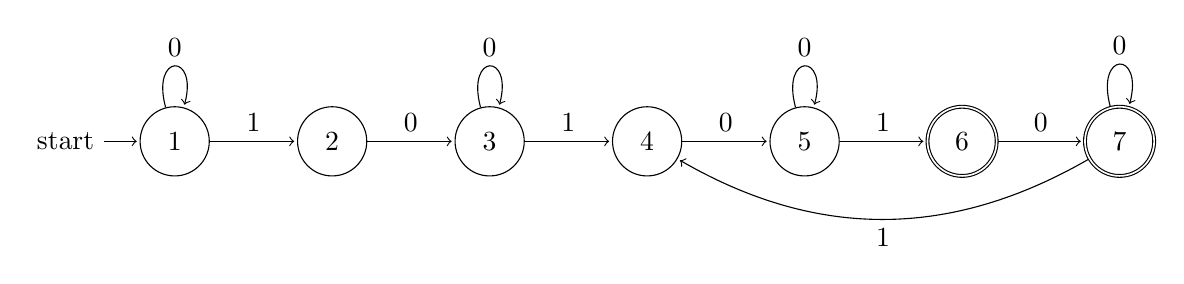
\begin{tikzpicture}[shorten >=1pt,node distance=2cm,on grid,auto]
        %% Your answer here
        \node[state,initial] (1)   {$1$};
        \node[state] (2) [right=of 1] {$2$};
        \node[state] (3) [right=of 2] {$3$};
        \node[state] (4) [right=of 3] {$4$};
        \node[state] (5) [right=of 4] {$5$};
        \node[state,accepting] (6) [right=of 5] {$6$};
        % \node[state] (5) [right=of 4] {$5$};
        \node[state,accepting](7) [right=of 6] {$7$};
        \path[->]
        (1) edge [loop above] node {$0$} ()
            edge  node  {1} (2)
        (2) edge  node  {0} (3)
            % edge [loop above] node {$\Sigma$} ()
        (3) edge  node  {1} (4)
            edge [loop above] node {$0$} ()
        (4) edge  node  {0} (5)
        (5) edge  node  {1} (6)
        edge [loop above] node {$0$} ()
        (6) edge  node  {0} (7)
        (7) edge [loop above] node {$0$} ()
        edge [bend left] node  {1} (4);
            % edge  node  {1} (6)
    \end{tikzpicture}
  \end{enumerate}

   \newpage


  \item \pts{$5\times 3=15$} Using the techniques covered in class, transform the following NFAs with $\epsilon$-transitions over the given alphabet $\Sigma$ into DFAs. Note that a DFA must have a transition defined for every state and symbol pair, whereas a NFA need not. You must take this fact into account for your transformations. Hint: Is there a subset of states the NFA transitions to when fed a symbol for which the set of current states has no explicit transition?

  \begin{enumerate}
    \item Original NFA, $\Sigma = \{a, b, c\}$:
    \\
    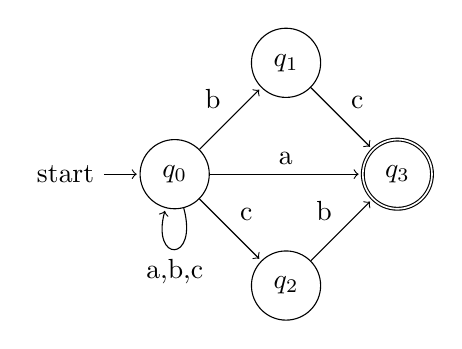
\begin{tikzpicture}[shorten >=1pt,node distance=2cm,on grid,auto]
        \node[state,initial] (q_0)   {$q_0$};
        \node[state] (q_1) [above right=of q_0] {$q_1$};
        \node[state] (q_2) [below right=of q_0] {$q_2$};
        \node[state,accepting](q_3) [below right=of q_1] {$q_3$};
        \path[->]
        (q_0) edge [loop below] node {a,b,c} ()
              edge  node  [above] {a} (q_3)
              edge  node  {b} (q_1)
              edge  node  {c} (q_2)
        (q_1) edge  node  {c} (q_3)
        (q_2) edge  node  {b} (q_3);
    \end{tikzpicture}
    \\
    DFA:
    \\
    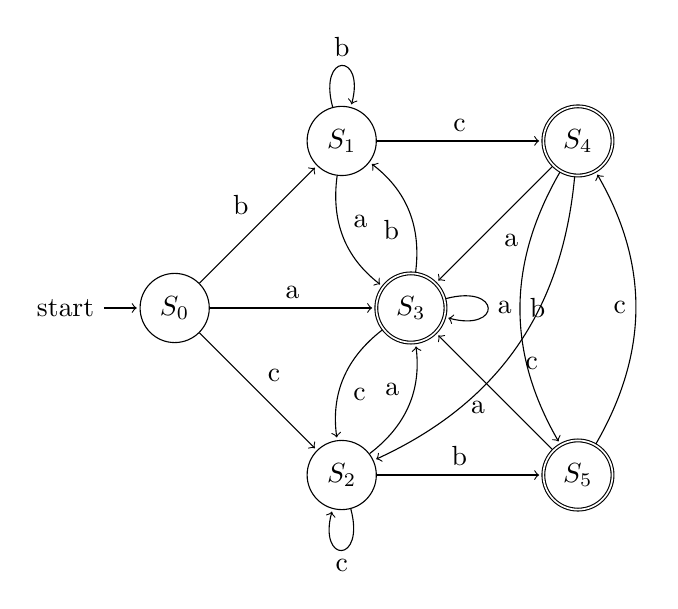
\begin{tikzpicture}[shorten >=1pt,node distance=3cm,on grid,auto]
        %% Your answer here
        \node[state,initial] (S_0)   {$S_0$};
        \node[state] (S_1) [above right=of S_0] {$S_1$};
        \node[state,accepting] (S_3) [right=of S_0] {$S_3$};
        \node[state] (S_2) [below right=of S_0] {$S_2$};
        \node[state,accepting](S_4) [right=of S_1] {$S_4$};
        \node[state,accepting](S_5) [right=of S_2] {$S_5$};
        \path[->]
        (S_0) %edge [loop below] node {a,b,c} ()
              edge  node  {a} (S_3)
              edge  node  {b} (S_1)
              edge  node  {c} (S_2)
        (S_1) edge [bend right] node  {a} (S_3)
        edge  node  {c} (S_4)
        edge [loop above] node {b} ()
        (S_2) edge  node  {b} (S_5)
        edge [bend right] node  {a} (S_3)
        edge [loop below] node {c} ()
        (S_3) edge [bend right] node  {c} (S_2)
        edge [bend right] node  {b} (S_1)
        edge [loop right] node {a} ()
        (S_4)% edge  node  {a} (S_5)
        edge [bend left] node  {c} (S_2)
        edge [bend right] node {b} (S_5)
        edge  node {a} (S_3)
        (S_5)edge [bend right] node  {c} (S_4)
        edge  node  {a} (S_3);
        % edge [loop above] node {a,c} ();
        
        %(S_6) edge  node  {a} (S_5)
        %edge  node  {b} (S_6)
        %edge [loop above] node {c} ()

    \end{tikzpicture}
    \\the origin is not elegant, So I replace it with the minimized version.

    \item Original NFA, $\Sigma = \{a, b, c\}$:
    \\
    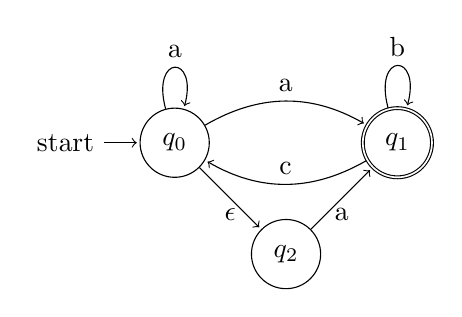
\begin{tikzpicture}[shorten >=1pt,node distance=2cm,on grid,auto]
        \node[state,initial] (q_0)   {$q_0$};
        \node[state] (q_2) [below right=of q_0] {$q_2$};
        \node[state,accepting] (q_1) [above right=of q_2] {$q_1$};
        \path[->]
        (q_0) edge [loop above] node {a} ()
              edge [bend left] node  {a} (q_1)
              edge  node [below] {$\epsilon$} (q_2)
        (q_1) edge [loop above] node {b} ()
              edge [bend left] node [above] {c} (q_0)
        (q_2) edge node [below] {a} (q_1);

        
    \end{tikzpicture}
    \\
    DFA:
    \\
    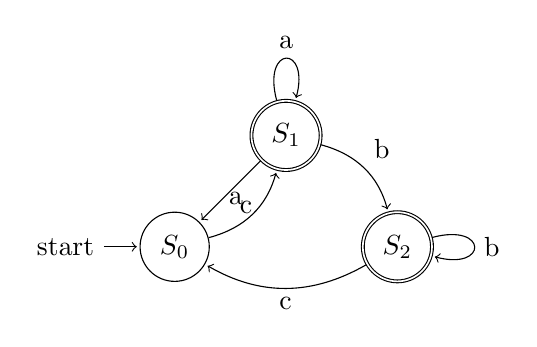
\begin{tikzpicture}[shorten >=1pt,node distance=2cm,on grid,auto]
                %% Your answer here
                \node[state,initial] (S_0)   {$S_0$};
                \node[state,accepting] (S_1) [above right=of S_0] {$S_1$};
                % \node[state] (S_3) [below right=of S_0] {$S_3$};
                \node[state,accepting](S_2) [below right=of S_1] {$S_2$};
                % \node[state,accepting](S_6) [below right=of S_4] {$S_6$};
                \path[->]
                (S_0) %edge [loop below] node {a,b,c} ()
                      edge [bend right] node  {a} (S_1)
                    %   edge  node  {b,c} (S_2)
                    %   edge  node  {c} (S_3)
                (S_1) edge [bend left] node  {b} (S_2)
                edge  node  {c} (S_0)
                edge [loop above] node {a} ()
                % (S_2) edge  node  {a} (S_2)
                % edge  node  {b,c} (S_4)
                % edge [loop above] node {b} ()
                
                (S_2) edge [bend left] node  {c} (S_0)
                % edge  node  {a} (S_4)
                edge [loop right] node {b} ();
                % (S_5)% edge  node  {a} (S_5)
                % edge  node  {b} (S_6)
                % edge [loop above] node {a,c} ();
                
                %(S_6) edge  node  {a} (S_5)
                %edge  node  {b} (\S_6)
                %edge [loop above] node {c} ()
    \end{tikzpicture}
    \\the origin is not elegant, So I replace it with the minimized version.
    \item Original NFA, $\Sigma = \{a, b,c\}$:
    \\
    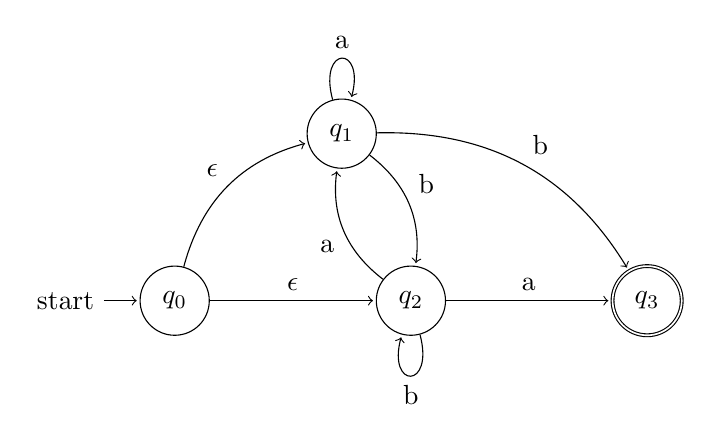
\begin{tikzpicture}[shorten >=1pt,node distance=3cm,on grid,auto]
        \node[state,initial] (q_0)   {$q_0$};
        \node[state] (q_1) [above right=of q_0] {$q_1$};
        \node[state] (q_2) [right=of q_0] {$q_2$};
        \node[state,accepting] (q_3) [right=of q_2] {$q_3$};
        \path[->]
        (q_0) edge [bend left] node  {$\epsilon$} (q_1)
              edge node  {$\epsilon$} (q_2)
        (q_1) edge [loop above] node {a} ()
              edge [bend left] node {b} (q_3)
              edge [bend left] node {b} (q_2)
        (q_2) edge [loop below] node {b} ()
              edge node {a} (q_3)
              edge [bend left] node {a} (q_1);
    \end{tikzpicture}
    \\
    DFA:
    \\
    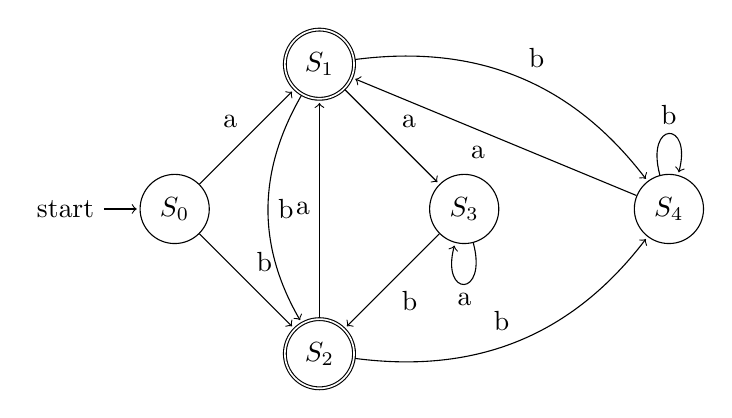
\begin{tikzpicture}[shorten >=1pt,node distance=2.6cm,on grid,auto]
        %% Your answer here
                %% Your answer here
                \node[state,initial] (S_0)   {$S_0$};
                \node[state,accepting](S_1) [above right=of S_0] {$S_1$};
                \node[state,accepting](S_2) [below right=of S_0] {$S_2$};
                \node[state](S_3) [below right=of S_1] {$S_3$};
                \node[state](S_4) [right=of S_3] {$S_4$};
                \path[->]
                (S_0) %edge [loop below] node {a,b,c} ()
                      edge  node  {a} (S_1)
                      edge  node  {b} (S_2)
                    %   edge  node  {c} (S_3)
                (S_1) edge [bend right] node  {b} (S_2)
                edge node  {a} (S_3)
                % edge  node  {c} (S_5)
                edge [bend left] node {b} (S_4) 
                (S_2) edge node  {a} (S_1)
                
                % edge [loop below] node {b} ()
                edge [bend right] node {b} (S_4)
                (S_3) 
                edge  node  {b} (S_2)
                % edge  node  {b} (S_6)
                edge [loop below] node {a} ()
                (S_4) edge node {a}(S_1)
                edge [loop above] node {b} ();

                % (S_4)% edge  node  {a} (S_5)
                % edge  node  {c} (S_6)
                % edge [loop above] node {a,b} ()
                
                % (S_5)% edge  node  {a} (S_5)
                % edge  node  {b} (S_6)
                % edge [loop above] node {a,c} ();
                
                %(S_6) edge  node  {a} (S_5)
                %edge  node  {b} (S_6)
                %edge [loop above] node {c} ()
    \end{tikzpicture}
  \end{enumerate}

   \newpage
  \item \pts{$13$}  Draw the NFA for the set of all strings over the alphabet $\Sigma = \{a,b\}$, where either $a$ occurs
  an odd number of times and each of pair of a is separated by exactly $2n+2$ consecutive b (for some $n \geq 0$), or $b$ occurs
  an even number of times and each of pair of relative consecutive b is separated by exactly $2m+1$ consecutive a (for some $m \geq 0$).
  Examples of strings that should be accepted by this NFA: abbabbbba, babaaabaaaaab.
  Examples of strings that should \textbf{not} be accepted: ababb, abbbabba.
    \\
    \\
    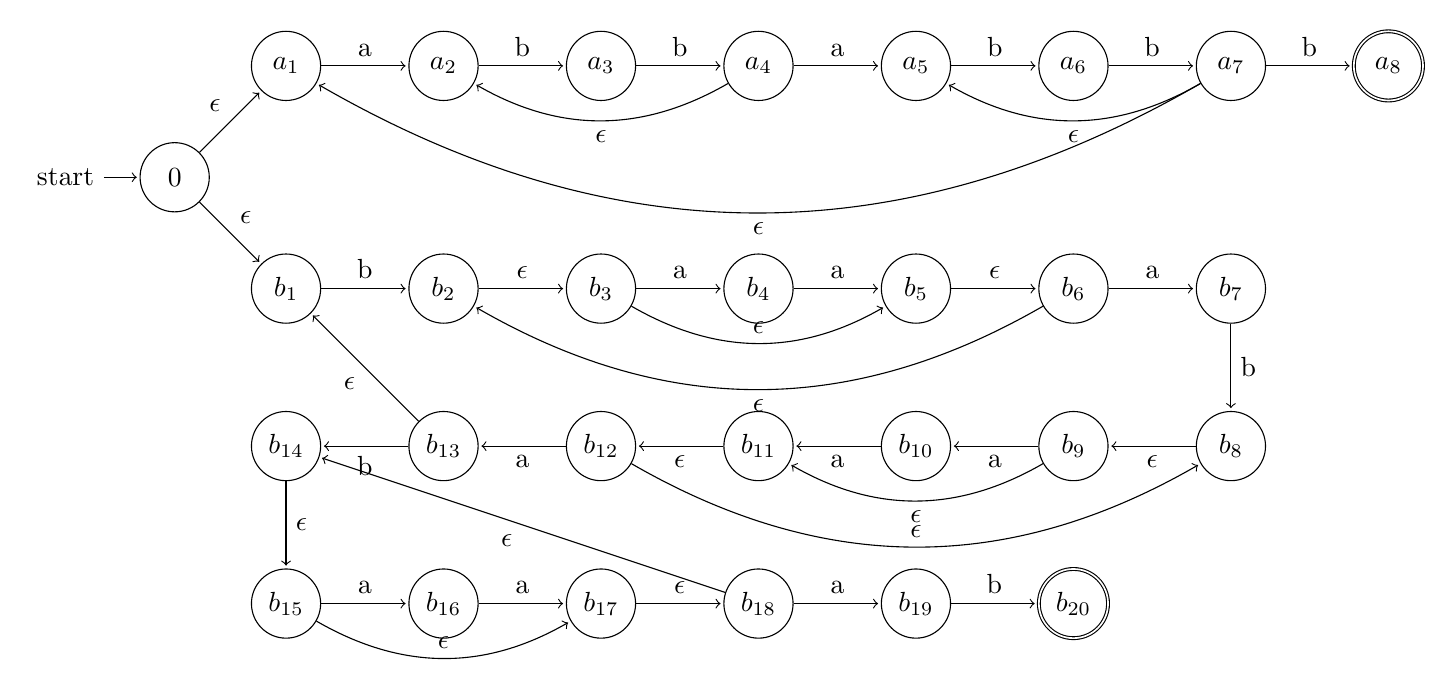
\begin{tikzpicture}[shorten >=1pt,node distance=2cm,on grid,auto]
 
            %% Your answer here
                    %% Your answer here
                    \node[state,initial] (0)   {$0$};
                    \node[state](a_1) [above right=of 0] {$a_1$};
                    \node[state](a_2) [right=of a_1] {$a_2$};
                    \node[state](a_3) [right=of a_2] {$a_3$};
                    \node[state](a_4) [right=of a_3] {$a_4$};
                    \node[state](a_5) [right=of a_4] {$a_5$};
                    \node[state](a_6) [right=of a_5] {$a_6$};
                    \node[state](a_7) [right=of a_6] {$a_7$};
                    \node[state,accepting](a_8) [right=of a_7] {$a_8$};
                    \node[state](b_1) [below right=of 0] {$b_1$};
                    \node[state](b_2) [right=of b_1] {$b_2$};
                    \node[state](b_3) [right=of b_2] {$b_3$};
                    \node[state](b_4) [right=of b_3] {$b_4$};
                    \node[state](b_5) [right=of b_4] {$b_5$};
                    \node[state](b_6) [right=of b_5] {$b_6$};
                    \node[state](b_7) [right=of b_6] {$b_7$};
                    \node[state](b_8) [below=of b_7] {$b_8$};
                    \node[state](b_9) [left=of b_8] {$b_9$};
                    \node[state](b_10) [left=of b_9] {$b_{10}$};
                    \node[state](b_11) [left=of b_10] {$b_{11}$};
                    \node[state](b_12) [left=of b_11] {$b_{12}$};
                    \node[state](b_13) [left=of b_12] {$b_{13}$};
                    \node[state](b_14) [left=of b_13] {$b_{14}$};
                    \node[state](b_15) [below=of b_14] {$b_{15}$};
                    \node[state](b_16) [right=of b_15] {$b_{16}$};
                    \node[state](b_17) [right=of b_16] {$b_{17}$};
                    \node[state](b_18) [right=of b_17] {$b_{18}$};
                    \node[state](b_19) [right=of b_18] {$b_{19}$};
                    \node[state,accepting](b_20) [right=of b_19] {$b_{20}$};
                    \path[->]
                    (0) %edge [loop below] node {a,b,c} ()
                          edge  node  {$\epsilon$} (a_1)
                          edge  node  {$\epsilon$} (b_1)
                        %   edge  node  {c} (S_3)
                    (a_1) edge  node  {a} (a_2)
                    (a_2) edge  node  {b} (a_3)
                    (a_3) edge  node  {b} (a_4)
                    (a_4) edge  node  {a} (a_5)
                    edge [bend left] node  {$\epsilon$} (a_2)
                    (a_5) edge  node  {b} (a_6)
                    (a_6) edge  node  {b} (a_7)
                    (a_7) edge  node  {b} (a_8)
                    edge [bend left] node  {$\epsilon$} (a_5)
                    edge [bend left] node  {$\epsilon$} (a_1)
                    (b_1) edge  node  {b} (b_2)
                    (b_2) edge  node  {$\epsilon$} (b_3)
                    (b_3) edge  node  {a} (b_4)
                    edge [bend right] node  {$\epsilon$} (b_5)
                    (b_4) edge  node  {a} (b_5)
                    % edge  node  {$\epsilon$} (a_2)
                    (b_5) edge  node  {$\epsilon$} (b_6)
                    (b_6) edge  node  {a} (b_7)
                    edge [bend left] node  {$\epsilon$} (b_2)
                    (b_7) edge  node  {b} (b_8)
                    (b_8) edge  node  {$\epsilon$} (b_9)
                    (b_9) edge  node  {a} (b_10)
                    edge [bend left] node  {$\epsilon$} (b_11)
                    (b_10) edge  node  {a} (b_11)
                    % edge  node  {$\epsilon$} (a_2)
                    (b_11) edge  node  {$\epsilon$} (b_12)
                    (b_12) edge  node  {a} (b_13)
                    edge [bend right] node  {$\epsilon$} (b_8)
                    (b_13) edge  node  {b} (b_14)
                    edge node  {$\epsilon$} (b_1)
                    (b_14) edge  node  {$\epsilon$} (b_15)
                    (b_15) edge  node  {a} (b_16)
                    edge [bend right] node  {$\epsilon$} (b_17)
                    (b_16) edge  node  {a} (b_17)
                    % edge  node  {$\epsilon$} (a_2)
                    (b_17) edge  node  {$\epsilon$} (b_18)
                    (b_18) edge  node  {a} (b_19)
                    edge  node  {$\epsilon$} (b_14)
                    (b_19) edge  node  {b} (b_20);
                    % (b_7) edge  node  {} (b_9)
                    % edge  node  {$\epsilon$} (a_16)
                    % edge  node  {$\epsilon$} (a_17)

                    % edge  node  {c} (S_5)
                    % edge [loop above] node {a} ()
                    % (S_2) edge [bend right] node  {a} (S_1)
                    % edge  node  {b} (S_3)
                    % edge [loop above] node {b} ()
                    
                    % (S_3) edge [bend left] node  {a} (S_1)
                    % % edge  node  {b} (S_6)
                    % edge [loop below] node {b} ();
                    
                    % (S_4)% edge  node  {a} (S_5)
                    % edge  node  {c} (S_6)
                    % edge [loop above] node {a,b} ()
                    
                    % (S_5)% edge  node  {a} (S_5)
                    % edge  node  {b} (S_6)
                    % edge [loop above] node {a,c} ();
                    
                    %(S_6) edge  node  {a} (S_5)
                    %edge  node  {b} (S_6)
                    %edge [loop above] node {c} ()
    \end{tikzpicture}

  \newpage
   \item Consider the following tokens and their associated regular expressions, given as a \textbf{flex} scanner specification:

  \begin{lstlisting}
    %%
    (if)                    {printf("IF");}
    [0-9]+                  {printf("NUM");}
    [a-zA-Z0-9]+            {printf("ID");}
    [ ]                     {}
  \end{lstlisting}

  Give an input to this scanner such that the output string is $\tt (IF^{\rm 2} ID^{\rm 3} NUM^{\rm 2})^{\rm 2}$, where $\tt A^i$ denotes {\tt A} repeated {\tt i} times.   (And, of course, the parentheses are not part of the output.)  You may use similar shorthand notation in your answer.
  \[
      if\; if\; aA9\; aA9\; aA9\; 9\; 9\; if\; if\; aA9\; aA9\; aA9\; 9\; 9\;
  \]

  \newpage
  \item Draw the minimal DFA of the DFA constructed in Question 4(c).
   \\
    \\
    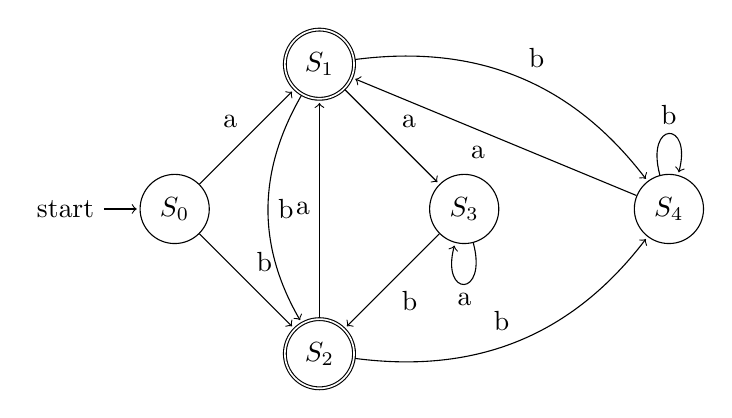
\begin{tikzpicture}[shorten >=1pt,node distance=2.6cm,on grid,auto]
        %% Your answer here
                %% Your answer here
                \node[state,initial] (S_0)   {$S_0$};
                \node[state,accepting](S_1) [above right=of S_0] {$S_1$};
                \node[state,accepting](S_2) [below right=of S_0] {$S_2$};
                \node[state](S_3) [below right=of S_1] {$S_3$};
                \node[state](S_4) [right=of S_3] {$S_4$};
                \path[->]
                (S_0) %edge [loop below] node {a,b,c} ()
                      edge  node  {a} (S_1)
                      edge  node  {b} (S_2)
                    %   edge  node  {c} (S_3)
                (S_1) edge [bend right] node  {b} (S_2)
                edge node  {a} (S_3)
                % edge  node  {c} (S_5)
                edge [bend left] node {b} (S_4) 
                (S_2) edge node  {a} (S_1)
                
                % edge [loop below] node {b} ()
                edge [bend right] node {b} (S_4)
                (S_3) 
                edge  node  {b} (S_2)
                % edge  node  {b} (S_6)
                edge [loop below] node {a} ()
                (S_4) edge node {a}(S_1)
                edge [loop above] node {b} ();

    \end{tikzpicture}

\end{enumerate}
\end{document}

